\section{6LoWPAN implementation in \mbox{Mote Runner}}
\begin{frame}[fragile]
  \frametitle{Introduction to 6LoWPAN}
  \begin{figure}
    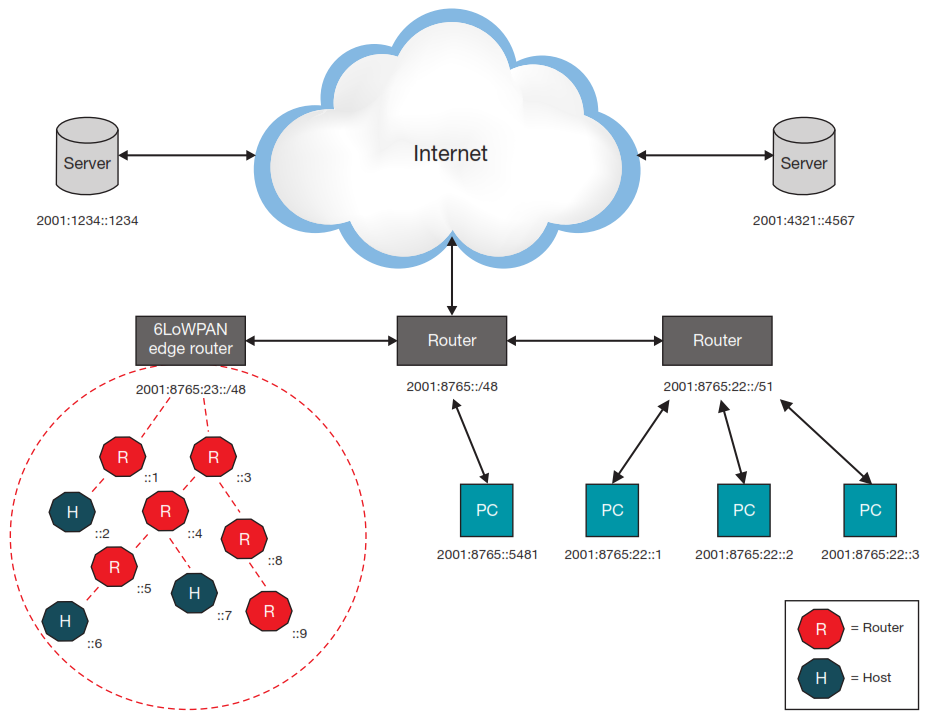
\includegraphics[width=.9\textwidth]{img/6low_network.png}
    \caption{IPv6 network with a 6LoWPAN mesh network}
  \end{figure}
\end{frame}

\begin{frame}[fragile]
  \frametitle{6LoWPAN stack}
  \begin{figure}
    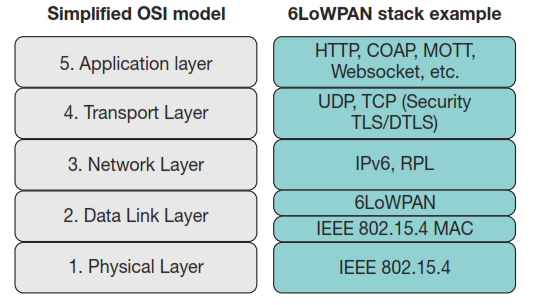
\includegraphics[width=.9\textwidth]{img/6low_stack.png}
  \end{figure}
\end{frame}

\begin{frame}[fragile]
  \frametitle{MRv6: an implementation of 6LoWPAN in MR}
  \begin{itemize}
    \item TDMA and beacon based multi-hop network which allows for an IPv6 based communication between motes
    \item Is not a bultin MR component, but fully implemented in C#
    \item Datagram packets exchanged adheres to a subset of th 6LoWPAN specifications
    \item The edge mote decides upon:
    \begin{itemize}
      \item Association requests
      \item Assigns communication schedules between wireless nodes
      \item Determines the routes in the network
    \end{itemize}
  \end{itemize}
\end{frame}

\begin{frame}[fragile]
  \frametitle{MRv6: Limitations}
  \begin{itemize}
    \item Only the transmission of UDP packets within the 6LoWPAN network is supported
    \item Exists only a proprietary broadcast operation to reach all motes in the network
    \item Is not suited for low latency application
    \item Does not support packet segmentation, reassembly and flow control
    \item Has been deployed in 900MHz or 2.4GHz frequency ranges and uses a single channel in the 2.4GHz band yet
  \end{itemize}
\end{frame}

\begin{frame}[fragile]
  \frametitle{Network Protocol}
  \begin{itemize}
    \item The network tree is only know to the edge
    \item The communication slots between parent and children are globally assigned by the edge and do never overlap
    \item At the beginning of their communication period parent motes send out beacon messages
    \begin{itemize}
      \item To synchronize the clock with their childrens
      \item To announce the state and schedule for the communication slots
    \end{itemize}
    \item Other then a fixed exclusive slot parent offers a shared slot (e.g. association requests and responses, broadcast messages)
    \item Beacon, shared and fixed slots form the superframe whose timings are assigned by the edge
  \end{itemize}
\end{frame}

\begin{frame}[Scheduling and Superframe]
  \frametitle{}
  \begin{figure}
    
\includegraphics[width=.9\textwidth]{img/6low_scheduling.png}
    \caption{Global schedule consists of a series of superframes}
  \end{figure}
  \begin{figure}
    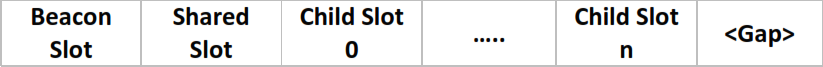
\includegraphics[width=.9\textwidth]{img/6low_superframe.png}
  \end{figure}
\end{frame}

\begin{frame}[Association and disassociation]
  \frametitle{}
  \begin{itemize}
    \item 
  \end{itemize}
\end{frame}

\begin{frame}[Data packets]
  \frametitle{}
  \begin{itemize}
    \item 
  \end{itemize}
\end{frame}